\documentclass[../../main]{subfiles}
\begin{document}
\section{Design and Development of the Drive Wheel and Gearbox System}


The following section is devoted to the design and development of the drive wheel and gearbox system, which is crucial for the mobility, stability, and functionality of the AGV.
The drive wheel and gearbox system is crucial in ensuring smooth and precise motion control, load handling, and adaptability to various operational environments. This project utilizes SolidWorks, a state-of-the-art computer-aided design software, for modeling and simulation of the drive wheel and gearbox. The robust tools for parametric design, assembly, and motion analysis in the software allow us to create an efficient and optimized design. It further takes into consideration practical constraints in reality, such as material selection, cost, manufacturability, environmental impact, and safety and engineering standards.
The objective of the project is to present a design that will not only be functional and reliable but also sustainable and economical. The successive sections outline the design process, engineering analysis, and critical decisions in view of the realization of the above-mentioned objectives in detail.

\subsection*{Key objectives included:}

\begin{itemize}
\item
  To design the system in SolidWorks.
\item
  Check for structural integrity at operational loads.
\item
  Analyze gearbox performance for the required torque and speed to
  achieve the desired gear ratio.
\item
  Simplify design for manufacturability and assembly.
\end{itemize}
\newpage
\section[Critical Elements of AGV Design]{Critical Elements of AGV Design: Drive Wheels, Gear Mechanisms, and Material Selection}

AGVs are driverless transport systems used in the manufacturing
industry, warehouses, and logistics. According to Groover (2015)\cite{groover2016automation}, in
"Automation, Production Systems, and Computer-Integrated Manufacturing"
an AGV would have a navigation system, a drive \\system, and sensors to
operate autonomously. The driving system is the major component of an
AGV, which provides the stability of the robot, the load-carrying
capability, and the accuracy of motion.

In AGVs, middle drive wheels are important for balance and drive.
Jazar\textquotesingle s study\cite{jazar2019road}, "Vehicle Dynamics: Theory and
Applications", presented in the year 2019, gave much \\importance to wheel
type, selection of motor, and gearbox that affects energy efficiency in
a robot, how much load a robot can carry, adaptation on various kinds of
terrain. A gearbox allows for the delivered torque and speed to the
wheel for smooth, accurate movement.

Research on gearbox design for robotics has highlighted the requirement
for compact, high-efficiency mechanisms. Kauffenberger et al. (2018)
studied gear mechanisms in small mobile robots and found that among
them, spur gears are the most used due to their simplicity, high load
capacity, and ease of manufacturing. Their study also discussed the
trade-off between gear ratios and torque output, noting that planetary
gear systems provide higher torque.

The design of the drive wheel is critical for traction, maneuverability,
and load-carrying capability. Bloss (2017), in "Mobile Robotics:
Principles and Design," has discussed the role of drive wheels in
robots, and he mentioned that material, tread pattern, and diameter of
the wheel have a direct influence on performance. The wheels for AGVs
are designed to meet both lightweight and high durability to allow for
continuous operation with various loads.

The CAD tools utilized for the design of robot systems are quite
popular, due to their advanced modeling and simulation capabilities. Das
and Jana 2020, in the work "Application of CAD Tools in Robotic Design",
have shown the capability of solid works to model complex assemblies
such as gearboxes and also to simulate their motions.

Material selection is one of the most critical aspects in mechanical
design. Ashby\cite{ashby1994materials}, 2011, "Materials Selection in Mechanical Design"
described a criterion for material selection that was based on strength,
weight, cost and environmental considerations. Since this project dealt
with drive wheels it mostly utilized rubberized materials, hence a thick
rubber material was chosen, while gears are made from hardened steel
preferred for its wear resistance and strength, it was also considered
in my material selection.

% \section{Design Constraints}
% \subsection{Technical Constraints}

% The following limitations relate to the feasibility and functionality of the design, encompassing several key factors:

% \begin{itemize}
%   \item 
%   Dimensional Accuracy: The dimensions need to be precise so that
%   the fitted parts inside assemble well.
  
%   \item 
%   Load Bearing Capacity: The wheels and gearbox should bear the
%   expected loads without deforming or failing.
  
%   \item 
%   Speed and Torque Requirements: The gear ratio and wheel design
%   must be such that desired performance is achieved.
  
%   \item 
%   Compatibility with Other Components: Ensure that the design fits
%   well with the AGV chassis, sensors, and other systems.
  
%   \item 
%   Assembly and Maintenance: The design must ensure ease assembly,
%   disassembly, and maintenance.
  
%   \item 
%   Simulation Accuracy: Limitations of CAD software may affect the
%   accuracy of stress, motion, or thermal simulations.
% \end{itemize}

% \subsection{Material Constraints}

% The choice of materials impacts weight, durability, and cost.
% \begin{itemize}
%   \item 
%   \textit{Strength and Durability:} Materials must be able to handle the
%   mechanical stresses without failure.
  
%   \item 
%   \textit{Weight:} Lighter materials are always preferred for efficiency,
%   but without sacrificing strength.
  
%   \item 
%   \textit{Availability}: Materials selected must be available to the
%   required quantity.
  
%   \item 
%   \textit{Cost}: The high-performance material may be beyond the budget and
%   therefore some compromise may be necessary.
% \end{itemize}
% Material selection for the drive wheels and gearbox is critical in balancing performance, cost, and durability. Gears and shafts were made from hardened steel due to its high strength and wear resistance, while aluminum alloys are preferred for wheel hubs and gearbox housings because of their lightweight and corrosion resistance. Drive wheel coatings were made from rubber or polyurethane to ensure traction, along with vibration absorption.
% The other alternatives, like plastics, are too weak and do not have enough strength to hold heavy loads; mild steel easily corrodes and is worn out, while on the other side, titanium, though very strong and light, is outrageously expensive and over-engineered for AGV applications. Materials selected ensure manufacturability with optimality, cost-effectiveness, and operation efficiency, making them the best choice for this project.

\section{Engineering Standards and Lifelong learning}
\subsection{Engineering standards}
Engineering standards provide a framework for designing, testing,
and manufacturing mechanical components to ensure compatibility, 
performance, safety, and reliability. Several organizations, such as 
ISO, ANSI, ASTM, IEEE, and DIN, define standards applicable to AGV drive systems.

\subsection{Importance of Engineering Standards in AGV Drive System Design}

Standards are essential in development to ensure:
\begin{itemize}
    \item \textit{Interoperability}: Components such as wheels, bearings, and shafts must conform to international sizes and tolerances. According to ISO 9001, which ensures a structured design and manufacturing process for reliability. 
    \item \textit{Safety}: Gearboxes and drive systems must adhere to safety regulations to prevent failures that could endanger users or disrupt operations. According to ISO 14121 ,  which helps in evaluating and mitigating risks associated with moving components.
    \item \textit{Manufacturing Feasibility}: Standardized materials and design practices facilitate efficient production and cost reduction. According to AGMA 2001-D04, which helps in designing gears that meet durability and performance requirements.
    \item \textit{Quality Assurance}: Standards define testing protocols for evaluating the durability and performance of components. According to ISO 606, which ensures proper gear-chain compatibility in AGV transmission systems.
\end{itemize}
\newpage
% \section{Manufacturing Constraints}

% The design should consider the limitations of manufacturing methods.

% Process Feasibility: The parts must be manufacturable using available
% processes such as CNC machining, casting or 3D printing.
% \begin{itemize}
%   \item 
%   \textit{Tool Accessibility:} Shapes that include internal grooves or
%   undercuts may not easily be machined due to complexity.
%   \item 

%   \textit{Surface Finish:} Very complicated surfaces may be expensive or
%   time-consuming to produce.
%   \item 

%   \textit{Assembly Difficulty:} Designs that include many parts or tight
%   clearances may be more difficult to assemble because of mating with
%   specific part which may not be possible if there are too tight.
%   \item 

%   \textit{Standard Components:} Using off-the-shelf components such as
%   bearings and shafts rather than customized components simplifies
%   production and reduces cost.
% \end{itemize}

% \section{Economic Constraints}

% In designing, fabricating, and deploying the driving wheels and gearboxes of an AGV, the main economic issues have to do with material type, manufacturing process, labor costs, maintenance, and scalability of the product.

% \begin{itemize}
%     \item \textit{Material Costs:} The use of high-performance materials, such as hardened steel and aluminum alloys, will enhance durability, but at increasingly higher costs. Using recycled or alternative materials may balance cost with performance.
    
%     \item \textit{Manufacturing Costs:} CNC machining, injection molding, and forging are cost-intensive to set up and hence affect the feasibility. Batch production and automation reduce the per-unit cost.
    
%     \item \textit{Labor and Skill Costs:} Skilled labor for design in SolidWorks, machining, and assembly increases the overall cost of the project. Automation and standardized components reduce labor dependence.
    
%     \item \textit{Maintenance and Lifecycle Costs:} Long-term costs are inclusive of the wear and tear of gears, battery efficiency, and availability for spares. Low-maintenance material selection and efficient motor designs reduce operational expenses.
    
%     \item \textit{Scalability and Mass Production:} Large-scale production reduces the unit cost due to bulk material discounts and streamlines the manufacturing process, though there is a requirement for high initial capital investment.
% \end{itemize}

% Lifecycle management can make the development of AGV drive systems cost-effective and green without compromising performance by applying optimization in design and manufacturing processes.

% \section{Environmental Constraints}

% Throughout their life, AGV drive wheels and gearboxes have some environmental impacts associated with each stage---from material extraction to end-of-life disposal. The most serious concerns are resource depletion, energy consumption, carbon footprint, and generation of wastes.

% \begin{itemize}
%     \item \textit{Material Impact:} The extraction and processing of steel, aluminum, and plastics lead to land degradation, energy usage, and air pollution. Recycled materials can be used in order to reduce the above-mentioned effects.
    
%     \item \textit{Manufacturing Waste:} Manufacturing processes involving CNC machining, injection molding, and heat treatment result in wastes like metal scraps, plastic wastes, and chemical by-products. The adoption of lean manufacturing and energy-efficient machinery reduces environmental degradation.
    
%     \item \textit{Energy Consumption \& Carbon Emissions:} AGVs use electric motors and batteries, and their production indirectly contributes to CO\(_2\) emissions if these are manufactured from fossil fuels. Efficient gearbox designs, regenerative braking, and renewable-powered charging stations could further improve sustainability.
    
%     \item \textit{Waste and Disposal Challenges:} Later in the life cycle, the components and batteries of AGVs pose waste challenges. Recycling programs, biodegradable lubricants, and modular component designs should be developed for environmental sustainability.
% \end{itemize}

% By the use of sustainable materials, manufacturing with a minimum of energy, and waste, the technology of AGV will go greener without losing efficiency and durability.

% \newpage
% \section{Health and Safety Problems}

% From both design and operational standpoints, the AGVs, their driving wheels, and gearboxes create many health and safety problems that have to be overcome to make them safe for workers and ensure reliability and operational efficiency. These aspects are very crucial in both the manufacturing process and final deployment within industrial environments. Thus, working out such problems would avoid accidents, injuries, and equipment failures.

% \begin{enumerate}
%     \item \textit{Manufacturing Hazards:} Workers are exposed to mechanical hazards, chemical exposure, and noise pollution. Safety measures include personal protective equipment, proper ventilation, and noise-reducing technologies.
    
%     \item \textit{Operational Safety Risks:} Gears can cause collisions, pinching, and crushing hazards, especially if visibility is poor. Safety measures involve collision avoidance systems, warning alarms, and clear design protocols.
    
%     \item \textit{Ergonomic Concerns:} Most of the assembly and maintenance tasks involve the risk of repetitive strain injuries and manual handling. This can be resolved by introducing automated handling systems, ergonomic tools, and workstations that are adjustable.
    
%     \item \textit{Hazards in Maintenance and Repair:} Maintenance involves workers in electrical risks, mechanical injuries, and harmful chemicals. These may be minimized by instituting lock-out/tag-out procedures, wearing PPE, and training in safe maintenance.
    
%     \item \textit{Long-term Health Issues:} Prolonged exposure to vibration, noise, and psychosocial stress can cause health problems such as hearing loss and vibration-induced problems. These risks can be minimized by regular health checks and stress management programs.
% \end{enumerate}

% By addressing these health and safety concerns, AGV manufacturers and operators can ensure a safer working environment, improve equipment reliability, and enhance overall worker well-being.
% \section{Manufacturability}

% Manufacturability refers to the development and production of the AGV drive wheels and gearboxes in an effective manner that is affordable and of great quality. Key considerations will include:

% \begin{enumerate}
%     \item \textit{Material Selection:} Lighter materials, such as aluminum, steel, and reinforced polymers, balance strength, wear resistance, and cost.
    
%     \item \textit{Design for Manufacturability:} Simplification of geometries, standardization of parts, modular design, and proper tolerancing enhance ease of fabrication and assembly.
    
%     \item \textit{Production Methods:} CNC machining, casting, forging, injection molding, and heat treatments are crucial for producing high-precision components efficiently.
    
%     \item \textit{Assembly Efficiency:} Reducing fastener types, using pre-assembled subcomponents, and integrating automated assembly speeds up production while maintaining consistency.
    
%     \item \textit{Cost and Scalability:} Choosing cost-effective production techniques, securing reliable supply chains, and optimizing mass production vs. small-batch production ensures economic feasibility.
    
%     \item \textit{Sustainability:} Using recyclable materials, energy-efficient manufacturing, waste reduction, and eco-friendly coatings supports environmentally responsible production.
% \end{enumerate}

% Therefore, focusing on these manufacturability aspects, manufacturers of AGVs can provide quality, durable, scalable drive wheels and gearboxes by optimizing cost, efficiency, and sustainability.


\section{Methodology}

The methodology followed for the project in brief is given below:

\begin{enumerate}
\def\labelenumi{\arabic{enumi}.}
\item
  Determination of dimensions, number of all gear teeth , and gear
  ratio.
\item
  3D Modeling: Detailed CAD modeling of wheels, gears, shafts, and
  housing on SolidWorks.
\item
  Simulation: motion analysis to validate the design.
\item
  Optimization: Refined design for performance and manufacturability.
\end{enumerate}

\subsection{Dimensions}

Ring gear which is the bigger gear has a dimater of 190 teeth

The planet gear has a diameter of 90mm

The sun gear has a diameter of 10mm
\begin{figure}[h]
  \centering
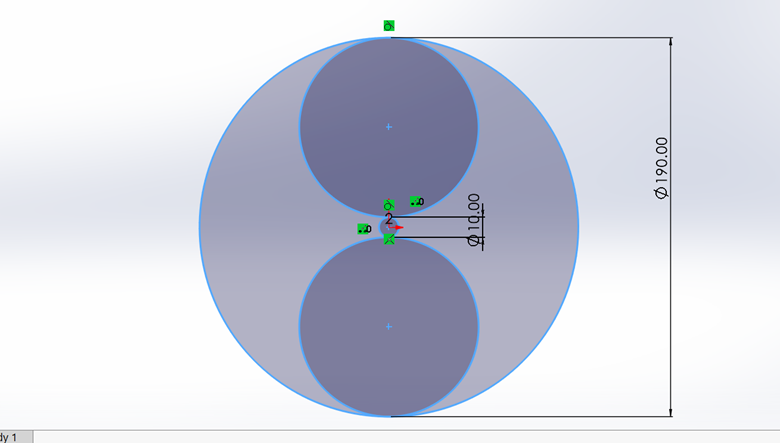
\includegraphics[width=\textwidth]{sublatex/Opryrmi/media/image1.png}
\caption{gear system dimensions}
\end{figure}

\newpage
\section{3D Modeling}

Following components were modelled using SolidWorks:



  \subsection{Middle Drive Wheels:}
  For Traction and load-carrying capacity. Which is
  made of natural rubber has the ability to withstand high load and
  relatively not so heavy. The wheels for AGVs are designed to meet both
  lightweight and high durability to allow for continuous operation with
  various loads.
  \begin{figure}[h]
    \centering
    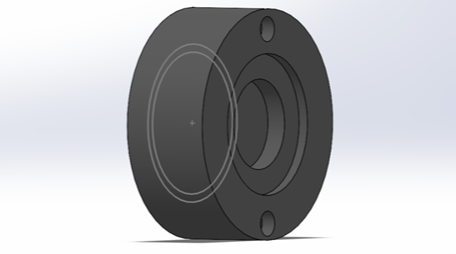
\includegraphics[width=0.8\textwidth]{sublatex/Opryrmi/media/image2.png} 
    \caption{Middle drive wheels made of natural rubber}
  \end{figure}



\subsection{Gearbox:}
Compact design with spur gears for efficient transmission.
Studies shows spur gears are the most used due to their simplicity, high
load capacity, and ease of manufacturing. Their study also discussed the
trade-off between gear ratios and torque output, noting that planetary
gear systems provide higher torque.
\begin{figure}[h]
  \centering
  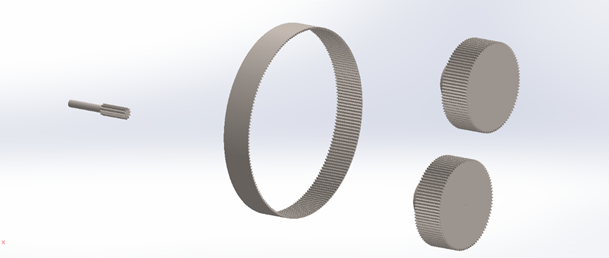
\includegraphics[width=0.8\textwidth]{sublatex/Opryrmi/media/image3.png} 
  \caption{Compact gearbox design}
\end{figure}

\subsection{Shafts and Bearings:} 
For smooth rotation and distribution of loads.
I made use of both skf bearing 108tn92 and skf bearing 1210ektn9202
while for the wheel holder it was made with hard steel for firmness and
durability.
\begin{figure}[h]
  \centering
  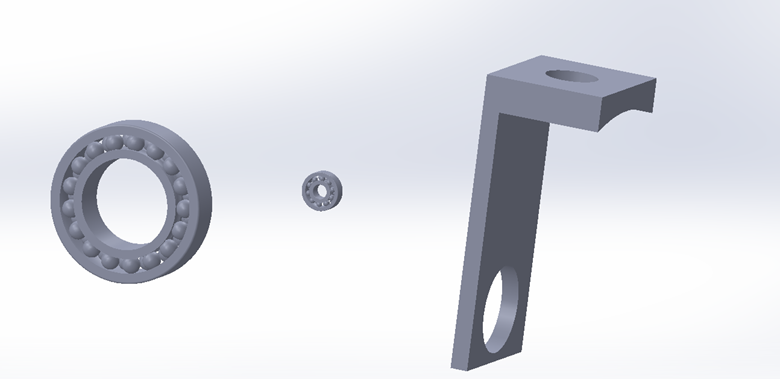
\includegraphics[width=0.8\textwidth]{sublatex/Opryrmi/media/image4.png} 
  \caption{Shafts and bearings assembly}
\end{figure}

\subsection{Housing:} 
Enclosed system for protection against dust and debris.
Which lightweight aluminum were used to reduce the weight of the gear
box.
\begin{figure}[h]
  \centering
  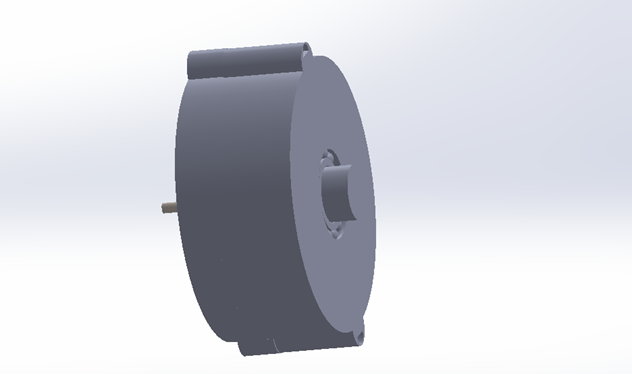
\includegraphics[width=0.8\textwidth]{sublatex/Opryrmi/media/image5.png} 
  \caption[Aluminum Housing for Dust Protection]{Enclosed housing made of lightweight aluminum for protection against dust and debris.}
\end{figure}

% \begin{figure}[ht]
%   \centering
%     \begin{subfigure}[b]{0.35\textwidth}
%         \centering
%         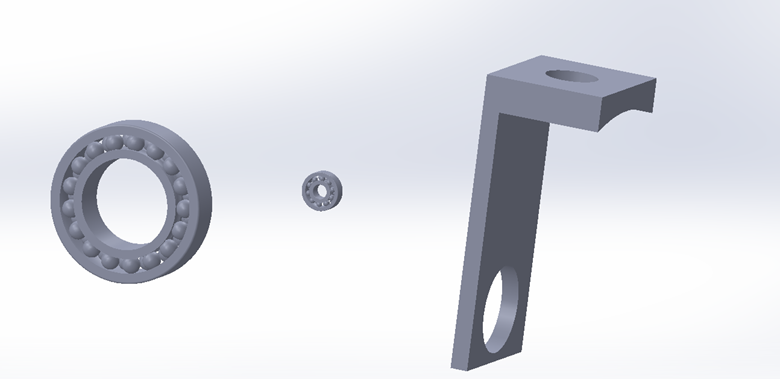
\includegraphics[width=\textwidth]{sublatex/Opryrmi/media/image4.png} 
%         \caption{Caption 1}
%     \end{subfigure}
%     \hspace{1em}
%     \begin{subfigure}[b]{0.45\textwidth}
%         \centering
%         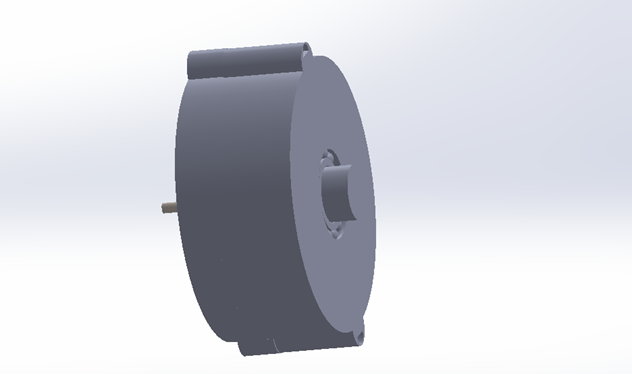
\includegraphics[width=\textwidth]{sublatex/Opryrmi/media/image5.png} 
%         \caption{Caption 2}
%     \end{subfigure}
%     \caption{Main caption for all images}
%     \label{fig:three_images}
% \end{figure}
\newpage
\subsection{Assembly}

The parts were then assembled in SolidWorks for a check on
appropriateness and \\ compatibility.
\begin{figure}[h]
  \centering
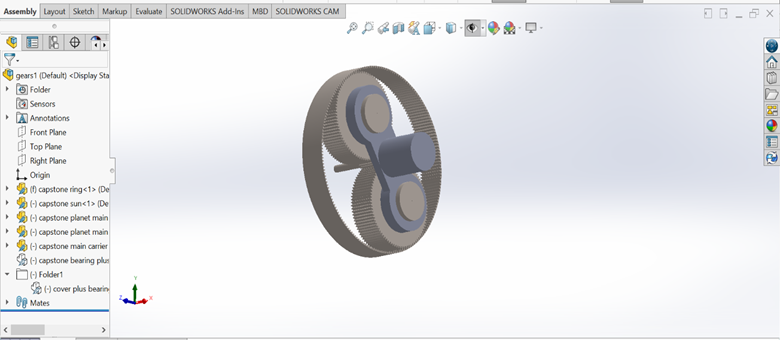
\includegraphics[]{sublatex/Opryrmi/media/image6.png}
\caption{}
\end{figure}

\section{Calculation and Analysis}

Simulations done in SolidWorks to test performances of the design:


\subsection{GEARBOX CALCULATION}


\begin{itemize}
\item
  ring gear \(\rightarrow 190\) Teeth {[}120 mm \(\phi\) {]} {[}Tr{]}
\item
  PLAMET Gear \(\rightarrow 90\) Teeth {[}Tp{]}
\item
  Sun gear \(\rightarrow 10\) Teeth {[}Ts{]}
\end{itemize}

GEAR RATIO : NOTE I want a high ratio of $20:1$

\[\begin{aligned}
  20 &= 1 + \cfrac{T_{r}}{T_{s}} \\
  \cfrac{T_{r}}{T_{s}} &= 19 \\
  T_{r} &= 19T_{s}
\end{aligned}\]

The planet does not affect the ratio but determines the spacing of the
sun and ring gears.
Rearanging:

\[\begin{aligned}
\frac{T_{r}}{T_{s}} &= 19 \\
IF\ T_{s} &= 10 \\
T_{r} &= 19 \times 10 = 190
\end{aligned}\]

from \(T_{r} - T_{s} = 2T_{p} \rightarrow\) Spacing in the ring

\[\begin{aligned}
190 - 10 &= 2T_{p} \\
T_{p} &= 90 \\
\ \to 1 + \frac{T_{r}}{T_{s}} &\Rightarrow 1 + \frac{190}{10} = 20 \\
\ \to &20:1
\end{aligned}\]

\(\to 1500\) input speed
\(\div 20(gear\ ratio) \Rightarrow 75rmp\) output speed

Considering\\
Nema 23 stepper motor\\
Nominal power \(\rightarrow 240\) Watts\\
Nominal voltage \(\rightarrow 484\)\\
Nominal current \(\rightarrow 5\text{ }A\)\\
Maminal rotation \(\rightarrow 1500rpm\)

\[T_{\text{in~}} = \frac{P \times 60}{2\pi \times N} = \frac{240 \times 60}{2\pi \times 1500} \Rightarrow T_{\text{in~}} = 1.53Nm\]

\begin{itemize}
\item
  This calalation is assumed \(100\%\) efficiency, Real - Idorly will be
  slightly lower due to losses {[}heat, friction{]}
\end{itemize}

\[\begin{aligned}
T_{\text{out~}}  \  &= T_{\text{in~}} \times R_{\text{atio~}} \times \eta\text{~~} \\
\  &= 1.53 \times 20 \times 0.94 \\
\  &= 28.2Nm
\end{aligned}\]

\[\begin{aligned}
\eta\lbrack\text{~efficiency~}\rbrack = \frac{\text{~Out put power~}}{\text{~Input poise~}} \times 100\% &= \frac{75 \times 28.2}{1500\  \times 1.53} \\
= \frac{2,115}{2,280} &= 0.927 = 92\%
\end{aligned}\]


\section{Motion Analysis:}

Wheels\textquotesingle{} rotation and torque transfer in the gearbox
simulated.

Result: Smooth motion with efficiency in power transmission.
\begin{figure}[h]
  \centering
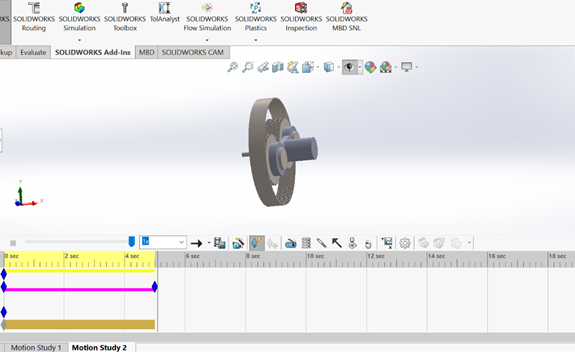
\includegraphics[]{sublatex/Opryrmi/media/image7.png}
\caption{}
\end{figure}

\emph{Material Selection}

\emph{Wheels}: Natural rubber, corrosion resistant and high load capacity.

\emph{Gears}: Hardened Steel for increased strength and wear resistance

\emph{Shafts}: Steel for durability

\emph{Housing}: aluminum protection


\end{document}